\documentclass[10pt]{article}
\usepackage[margin=1.0cm]{geometry}
\usepackage[T1]{fontenc}
\usepackage{lmodern}
\usepackage{xcolor}
\usepackage{tikz}
\usepackage{pgfplots}
\usepgfplotslibrary{statistics}
\pgfplotsset{compat=1.18}
\definecolor{srblue}{HTML}{2F6B9A}
\definecolor{opencvorange}{HTML}{D97706}
\definecolor{fps2blue}{HTML}{B9D7EA}
\definecolor{fps5orange}{HTML}{F6C28B}
\definecolor{stslightgreen}{HTML}{A7D8B1}
\definecolor{stsstronggreen}{HTML}{208B3A}
\definecolor{sugarlightpurple}{HTML}{CBB7E8}
\definecolor{sugarstrongpurple}{HTML}{763A9B}
\definecolor{stsedge}{HTML}{1D4E89}
\definecolor{sugaredge}{HTML}{B45309}
\definecolor{incompletegray}{HTML}{9CA3AF}
\definecolor{deltared}{HTML}{B91C1C}
\definecolor{deltagreen}{HTML}{15803D}
\newcommand{\legendcircle}[1]{\tikz[baseline=-0.6ex]\node[draw=black,fill=#1,circle,minimum size=4.5pt,inner sep=0pt] {};}
\newcommand{\legendsquare}[1]{\tikz[baseline=-0.6ex]\node[draw=black,fill=#1,rectangle,minimum size=4.5pt,inner sep=0pt] {};}
\newcommand{\legendtriangle}[1]{\tikz[baseline=-0.6ex]\draw[draw=black,fill=#1,line width=0.4pt] (0,2.3pt)--(-2.3pt,-1.8pt)--(2.3pt,-1.8pt)--cycle;}
\begin{document}
\pagestyle{empty}
\begin{center}
{\Large\bfseries SuGaR-Coarse-9000: objektmaskierte Bildmetriken}\\[3pt]
{\small Explorative Darstellung; Laufzeit = vollständiger archivierter Pipeline-Lauf}\\[8pt]
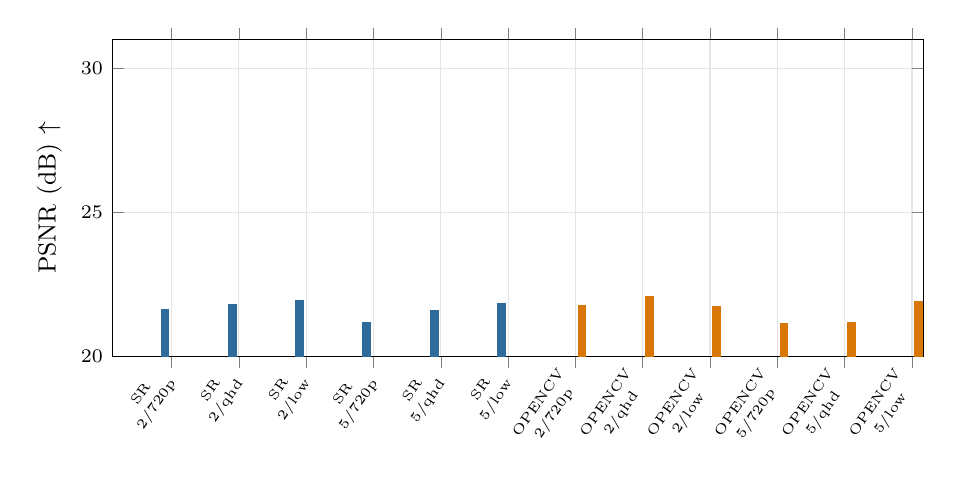
\begin{tikzpicture}
\begin{axis}[height=5.6cm,width=0.98\linewidth,ybar,bar width=2.8pt,enlarge x limits=0.015,xmin=-0.7,ymin=20,ymax=31,xtick=data,xticklabels={{\shortstack{SR\\2/720p}},{\shortstack{SR\\2/qhd}},{\shortstack{SR\\2/low}},{\shortstack{SR\\5/720p}},{\shortstack{SR\\5/qhd}},{\shortstack{SR\\5/low}},{\shortstack{OPENCV\\2/720p}},{\shortstack{OPENCV\\2/qhd}},{\shortstack{OPENCV\\2/low}},{\shortstack{OPENCV\\5/720p}},{\shortstack{OPENCV\\5/qhd}},{\shortstack{OPENCV\\5/low}}},x tick label style={font=\tiny,rotate=55,anchor=east},ylabel style={font=\small},tick label style={font=\scriptsize},ylabel={PSNR (dB) $\uparrow$},grid=major,grid style={gray!20},xtick={0,1,2,3,4,5,6,7,8,9,10,11}]
\addplot+[fill=srblue,draw=srblue,area legend] coordinates {(0,21.60365263) (1,21.80344288) (2,21.94173862) (3,21.15583377) (4,21.57142085) (5,21.83137436)};
\addplot+[fill=opencvorange,draw=opencvorange,area legend] coordinates {(6,21.77515639) (7,22.08118374) (8,21.72007820) (9,21.12995336) (10,21.16734883) (11,21.89677851)};
\end{axis}
\end{tikzpicture}
\par\vspace{2pt}
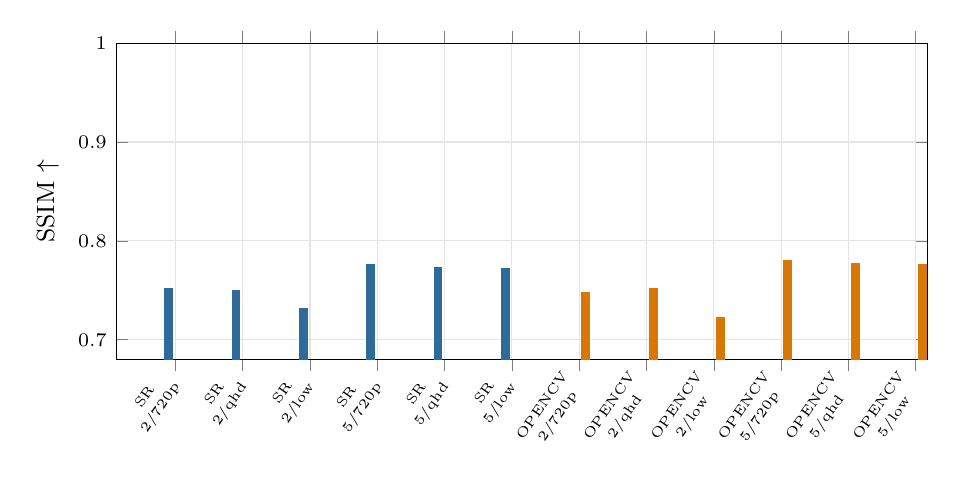
\begin{tikzpicture}
\begin{axis}[height=5.6cm,width=0.98\linewidth,ybar,bar width=2.8pt,enlarge x limits=0.015,xmin=-0.7,ymin=0.68,ymax=1.0,xtick=data,xticklabels={{\shortstack{SR\\2/720p}},{\shortstack{SR\\2/qhd}},{\shortstack{SR\\2/low}},{\shortstack{SR\\5/720p}},{\shortstack{SR\\5/qhd}},{\shortstack{SR\\5/low}},{\shortstack{OPENCV\\2/720p}},{\shortstack{OPENCV\\2/qhd}},{\shortstack{OPENCV\\2/low}},{\shortstack{OPENCV\\5/720p}},{\shortstack{OPENCV\\5/qhd}},{\shortstack{OPENCV\\5/low}}},x tick label style={font=\tiny,rotate=55,anchor=east},ylabel style={font=\small},tick label style={font=\scriptsize},ylabel={SSIM $\uparrow$},grid=major,grid style={gray!20},xtick={0,1,2,3,4,5,6,7,8,9,10,11}]
\addplot+[fill=srblue,draw=srblue,area legend] coordinates {(0,0.75188178) (1,0.74990743) (2,0.73163200) (3,0.77630728) (4,0.77305094) (5,0.77199414)};
\addplot+[fill=opencvorange,draw=opencvorange,area legend] coordinates {(6,0.74740580) (7,0.75128989) (8,0.72197089) (9,0.77968981) (10,0.77716404) (11,0.77627132)};
\end{axis}
\end{tikzpicture}
\par\vspace{2pt}
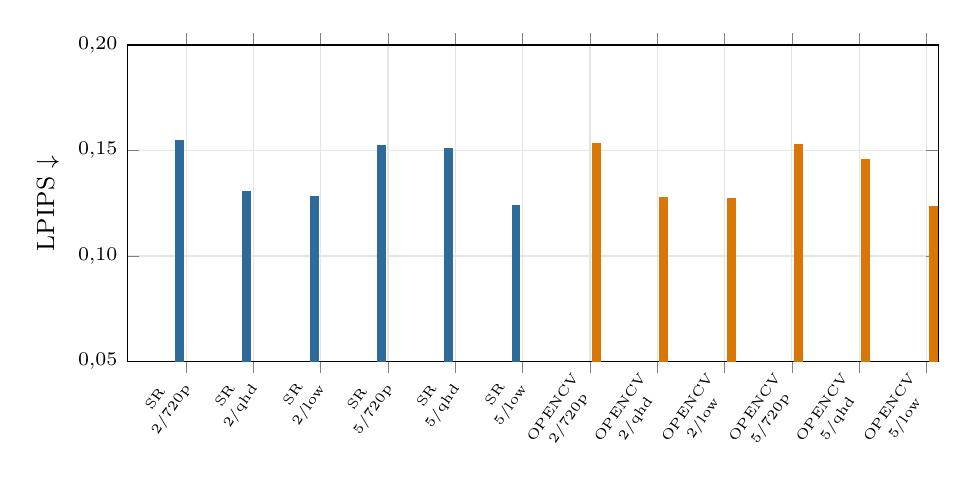
\begin{tikzpicture}
\begin{axis}[height=5.6cm,width=0.98\linewidth,ybar,bar width=2.8pt,enlarge x limits=0.015,xmin=-0.7,ymin=0.05,ymax=0.2,xtick=data,xticklabels={{\shortstack{SR\\2/720p}},{\shortstack{SR\\2/qhd}},{\shortstack{SR\\2/low}},{\shortstack{SR\\5/720p}},{\shortstack{SR\\5/qhd}},{\shortstack{SR\\5/low}},{\shortstack{OPENCV\\2/720p}},{\shortstack{OPENCV\\2/qhd}},{\shortstack{OPENCV\\2/low}},{\shortstack{OPENCV\\5/720p}},{\shortstack{OPENCV\\5/qhd}},{\shortstack{OPENCV\\5/low}}},x tick label style={font=\tiny,rotate=55,anchor=east},ylabel style={font=\small},tick label style={font=\scriptsize},ylabel={LPIPS $\downarrow$},grid=major,grid style={gray!20},scaled y ticks=false,ytick={0.05,0.10,0.15,0.20},yticklabels={{0,05},{0,10},{0,15},{0,20}},xtick={0,1,2,3,4,5,6,7,8,9,10,11}]
\addplot+[fill=srblue,draw=srblue,area legend] coordinates {(0,0.15454567) (1,0.13049116) (2,0.12839596) (3,0.15229463) (4,0.15094676) (5,0.12377006)};
\addplot+[fill=opencvorange,draw=opencvorange,area legend] coordinates {(6,0.15349434) (7,0.12767535) (8,0.12735538) (9,0.15278799) (10,0.14565088) (11,0.12357728)};
\end{axis}
\end{tikzpicture}
\par\vspace{2pt}
\vspace{3pt}
\begin{minipage}{0.98\linewidth}\scriptsize Alle zwölf Balkenpaare stammen aus \texttt{sugar\_coarse\_masked.json}; die STS-Baseline wird nicht als SuGaR-Ergebnis verwendet. PSNR/SSIM: höher ist besser; LPIPS: niedriger ist besser.\end{minipage}
\end{center}
\end{document}